\section{Physical access structures}

\begin{definition}[\textit{Access methods}]
    The access methods are software modules that provide data access and manipulation primitives for each physical data structure. 
\end{definition}
Each DBMS has a distinctive and limited set of access methods. 
These methods employ specific data structures to organize data, with each table being stored in precisely one primary physical data structure, and potentially having one or more optional secondary access structures.

\paragraph*{Classification}
These structures are categorized into: 
\begin{itemize}
    \item \textit{Primary structure}: contains all the tuples of a table. 
        Its primary purpose is to store the table content. 
    \item \textit{Secondary structures}: used to index primary structures, they only contain the values of certain fields interleaved with pointers to the blocks of the primary structure. 
    Their primary function is to accelerate the search for specific tuples based on designated search criteria.
\end{itemize}
Three main types of data access structures exist: sequential, hash-based, and tree-based.
\begin{table}[H]
    \centering
    \begin{tabular}{c|cc|}
    \cline{2-3}
                                                         & \textbf{Primary} & \textbf{Secondary} \\ \hline
    \multicolumn{1}{|c|}{\textbf{Sequential structures}} & Typical          & Not used           \\
    \multicolumn{1}{|c|}{\textbf{Hash-based structures}} & In some DBMS     & Frequent           \\
    \multicolumn{1}{|c|}{\textbf{Tree-based structures}} & Rare             & Typical            \\ \hline
    \end{tabular}
\end{table}

\paragraph*{Blocks and tuples}
Blocks serve as the physical components of files, while tuples are the logical components of tables.
The block size is usually fixed and depends on the file system and disk formatting, whereas the tuple size (also known as a record) is variable within a file and contingent on the database design.
For sequential and hash-based methods, a block is subdivided into the following components:
\begin{itemize}
    \item Block header and trailer containing control information utilized by the File System.
    \item Page header and trailer with control information related to the access method. 
    \item Page dictionary comprising pointers to each elementary item of useful data within the page.
    \item A useful part containing the data. 
    \item Typically, page dictionaries and useful data expand as a stack in opposite directions.
    \item A checksum to verify the integrity of the block.
\end{itemize}
\begin{figure}[H]
    \centering
    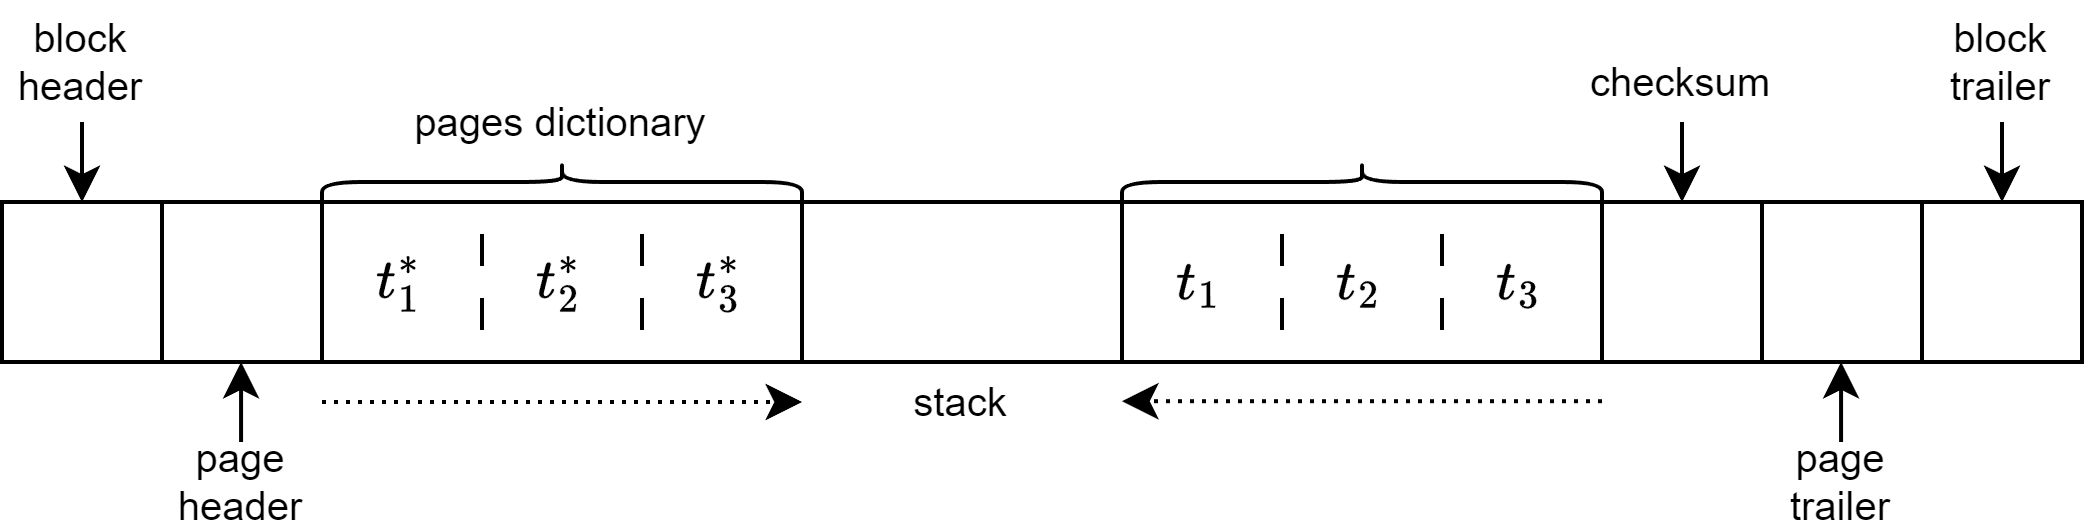
\includegraphics[width=0.75\linewidth]{images/block.png}
    \caption{Structure of a block}
\end{figure} 
The block factor ($B$) denotes the number of tuples within a block. 
To assess query costs, the following information is required:
\begin{itemize}
    \item SR: the average size of a record (or tuple). 
    \item SB: the average size of a block. 
\end{itemize}
The block factor is defined as:
\[B=\left\lfloor \dfrac{\text{SB}}{\text{SR}} \right\rfloor \]
The remaining space can either be used, if the records are spanned between blocks, or not used if the records are unspanned.

\paragraph*{Buffer manager}
Operations are executed in main memory and impact pages.
In our cost model we assume pages of equal size and organization as blocks. 
The buffer operations encompass:
\begin{itemize}
    \item \textit{Insertion} and update of a tuple: may require a reorganization of the page or usage of a new page, also update to a field may require reorganization.
    \item \textit{Deletion} of a tuple: typically accomplished by marking the tuple as invalid, with subsequent reorganization of the page performed asynchronously.
    \item \textit{Access} to a field of a particular tuple: identified according to an offset with respect to the beginning of the tuple and the length of the field itself.
\end{itemize}

\subsection{Sequential structures}
In the context of sequential structures, we encounter an ordered arrangement of tuples in secondary memory, allowing for efficient access to the next element. 
Blocks can be either contiguous on disk or sparse. 
Two main possibilities arise:
\begin{itemize}
    \item \textit{Entry-sequenced organization}: sequence of tuples dictated by their order of entry. 
    \item \textit{Sequentially-ordered organization}: tuples ordered according to the value of a key. 
\end{itemize}

\paragraph*{Entry-sequenced organization}
Entry-sequenced organization, also known as a heap, represents the simplest and most common type of sequential organization. 
This organization proves to be efficient for:
\begin{itemize}
    \item Insertion: this operation does not require shifting. 
    \item Space occupancy: it utilizes all available blocks for data and all the space within a block.
    \item Sequential reading and writing: especially advantageous if the blocks are contiguous.
    \item Query like \texttt{SELECT * FROM table}. 
\end{itemize}
However, it is inefficient for:
\begin{itemize}
    \item Searching specific data units: this may require scanning the entire structure, a challenge mitigated by using indexes.
    \item Updates that increase tuple size: this may necessitate shifting and writing to another block. 
        Deleting old versions of tuples and inserting new ones can address this issue.
    \item Query like \texttt{SELECT * FROM table WHERE <condition>}.
\end{itemize}

\paragraph*{Sequentially-ordered sequential structure}
In this organization, tuples are sorted based on the value of a key field. 
It is efficient for:
\begin{itemize}
    \item Range queries: retrieving tuples with the key in a specified interval.
    \item \texttt{ORDER BY} and \texttt{GROUP BY} queries: exploiting the key for sorting and grouping.
\end{itemize}
However, it is inefficient for reordering tuples within a block, especially challenging if space is limited.
To address the global reordering issue, various techniques can be employed:
\begin{itemize}
    \item Differential files and periodic merging.
    \item Local reordering operation within a block.
    \item Creation of an overflow file that contains tuples that do not fit in the current block. 
\end{itemize}

\paragraph*{Summary}
In real-world applications, the entry-sequenced organization is the most common solution only if paired with secondary access structures.
\begin{table}[H]
    \centering
    \begin{tabular}{l|ll|}
    \cline{2-3}
    \textbf{}                                                         & \textbf{Entry sequenced} & \textbf{Sequentially ordered} \\ \hline
    \multicolumn{1}{|l|}{\texttt{INSERT}}                             & Efficient                & Not efficient                 \\
    \multicolumn{1}{|l|}{\texttt{UPDATE}}                             & Efficient                & Not efficient                 \\
    \multicolumn{1}{|l|}{\texttt{DELETE}}                             & Invalid                  & Invalid                       \\
    \multicolumn{1}{|l|}{Tuple size}                                  & Fixed or variable        & Fixed or variable             \\
    \multicolumn{1}{|l|}{\texttt{SELECT * FROM T WHERE <condition>}}  & Not efficient            & Efficient                     \\ \hline
    \end{tabular}
\end{table}

\subsection{Hash-based structures}
Hash-based access structures provide efficient associative access to data based on the value of a key. 
The structure comprises $N_B$ buckets ($N_B \ll$ number of data items), with each bucket being a unit of storage, typically equivalent to the size of one block. 
These buckets are often stored adjacently in the file.

A hash function maps the key field to a value between 0 and $N_B-1$, interpreted as the index of a bucket in the hash structure (hash table). 
This organization proves efficient for:
\begin{itemize}
    \item Tables with small size and (almost) static content. 
    \item Point queries: queries with equality predicates on the key.
\end{itemize}
However, it is inefficient for:
\begin{itemize}
    \item Range queries and full table queries.
    \item Tables with highly dynamic content.
\end{itemize}

\paragraph*{Hash function}
The implementation of the hash function consists of two parts:
\begin{enumerate}
    \item \textit{Folding}: transforms key values into positive integer values, uniformly distributed over a large range.
    \item \textit{Hashing}: transforms the positive number into a value between $0$ and $N_B-1$ to identify the appropriate bucket for the tuple.
\end{enumerate}

\paragraph*{Collisions}
Collisions occur when two keys (tuples) are associated with the same bucket. 
When the maximum number of tuples per block is exceeded, collision resolution techniques are applied:
\begin{itemize}
    \item \textit{Closed hashing (open addressing)}: tries to find a slot in another bucket in the hash table.
        Linear probing is a simple technique, but not commonly used in databases.
    \item \textit{Open hashing (separate chaining)}: allocates a new bucket for the same hash result, linked to the previous one.
\end{itemize}
Finding a tuple corresponding to a given key typically requires one access, although occasionally more. 

\paragraph*{Overflow chain}
The cost of accessing the tuple can be estimated by considering the average length of the overflow chain, which is influenced by:
\begin{itemize}
    \item The load factor, that is the ratio of the occupied slots over the available slots:
        \[\dfrac{T}{B \cdot N_B}\]
    \item The block factor $B$. 
\end{itemize}
Here, $T$ is the number of tuples, $N_B$ is the number of buckets, and $B$ is the number of tuples within a block. 
The average of accesses to the overflow list is summarized in the following table: 
\begin{table}[H]
    \centering
    \begin{tabular}{ccccccc}
                                                               & \textit{}                         & \multicolumn{5}{c}{\textbf{Block factor}}                                                                                                                               \\ \cline{3-7} 
    \textit{}                                                  & \multicolumn{1}{c|}{}             & \multicolumn{1}{c|}{\textit{1}} & \multicolumn{1}{c|}{\textit{2}} & \multicolumn{1}{c|}{\textit{3}} & \multicolumn{1}{c|}{\textit{4}} & \multicolumn{1}{c|}{\textit{5}} \\ \cline{2-7} 
    \multicolumn{1}{c|}{\multirow{5}{*}{\textbf{Load factor}}} & \multicolumn{1}{c|}{\textit{50\%}} & \multicolumn{1}{c|}{0.5}        & \multicolumn{1}{c|}{0.177}      & \multicolumn{1}{c|}{0.087}      & \multicolumn{1}{c|}{0.031}      & \multicolumn{1}{c|}{0.005}      \\ \cline{2-7} 
    \multicolumn{1}{c|}{}                                      & \multicolumn{1}{c|}{\textit{60\%}} & \multicolumn{1}{c|}{0.75}       & \multicolumn{1}{c|}{0.293}      & \multicolumn{1}{c|}{0.158}      & \multicolumn{1}{c|}{0.066}      & \multicolumn{1}{c|}{0.015}      \\ \cline{2-7} 
    \multicolumn{1}{c|}{}                                      & \multicolumn{1}{c|}{\textit{70\%}} & \multicolumn{1}{c|}{1.167}      & \multicolumn{1}{c|}{0.494}      & \multicolumn{1}{c|}{0.286}      & \multicolumn{1}{c|}{0.136}      & \multicolumn{1}{c|}{0.042}      \\ \cline{2-7} 
    \multicolumn{1}{c|}{}                                      & \multicolumn{1}{c|}{\textit{80\%}} & \multicolumn{1}{c|}{2.0}        & \multicolumn{1}{c|}{0.903}      & \multicolumn{1}{c|}{0.554}      & \multicolumn{1}{c|}{0.289}      & \multicolumn{1}{c|}{0.110}      \\ \cline{2-7} 
    \multicolumn{1}{c|}{}                                      & \multicolumn{1}{c|}{\textit{90\%}} & \multicolumn{1}{c|}{4.495}      & \multicolumn{1}{c|}{2.146}      & \multicolumn{1}{c|}{1.377}      & \multicolumn{1}{c|}{0.777}      & \multicolumn{1}{c|}{0.345}      \\ \cline{2-7} 
    \end{tabular}
\end{table}
\begin{example}
    For an operation with a block factor of three and a load factor of seventy percent, the table indicates an average of 0.286 accesses to the overflow list. 
    Consequently, the number of I/O operations is approximately 1.3.
\end{example} 

\paragraph*{Indexing}
Hash-based structures can be employed for secondary indexes, shaped and managed like a hash-based primary structure. 
Instead of tuples, the buckets only contain key values and pointers.
Indexing without an overflow chain incurs a minimum cost of 2 I/O operations.

\paragraph*{Summary}
In a large database, searching all index values to reach the desired data is inefficient. 
Hash-based structures exhibit good performance for equality predicates on the key field but prove inefficient for access based on interval predicates or the value of non-search-key attributes.

\subsection{Indexes}
Indexes are data structures designed to efficiently retrieve tuples based on specific criteria, known as a search key.
Index entries are sorted with respect to the search key and typically contain records in the form 
\[\left\langle \text{search key}, \text{pointer to block}\right\rangle \]

\paragraph*{Primary and search keys}
It's crucial to distinguish between the primary key, used for uniquely identifying a tuple, and the search key, employed for retrieving tuples based on specific criteria.
\begin{table}[H]
    \centering
    \begin{tabular}{c|cc|}
    \cline{2-3}
                                                           & \textbf{Primary key} & \textbf{Search key} \\ \hline
    \multicolumn{1}{|c|}{\textbf{Access path defined}}     & $\tikzxmark$         & $\checkmark$        \\
    \multicolumn{1}{|c|}{\textbf{Constraint defined}}      & $\checkmark$         & $\tikzxmark$        \\
    \multicolumn{1}{|c|}{\textbf{Unique}}                  & $\checkmark$         & $\tikzxmark$        \\
    \multicolumn{1}{|c|}{\textbf{Implementation by index}} & $\checkmark$         & $\tikzxmark$        \\ \hline
    \end{tabular}
\end{table}

\paragraph*{Index classification}
Indexes are smaller than primary data structures and can be loaded into a file in the main memory.
They efficiently support point queries, range queries, and sorted scans. 
However, adding indexes to tables requires the DBMS to update each index after an insert, update, or delete operation, which can be costly and may slow down operations.

\begin{definition}[\textit{Dense index}]
    An index is considered dense when it has an index entry for each search-key value in the file (one index per tuple). 
\end{definition}
This type of index provides excellent performance since a search on the index is sufficient to access the correct tuple. 
Dense indexing is applicable to entry-sequenced primary structures.
\begin{figure}[H]
    \centering
    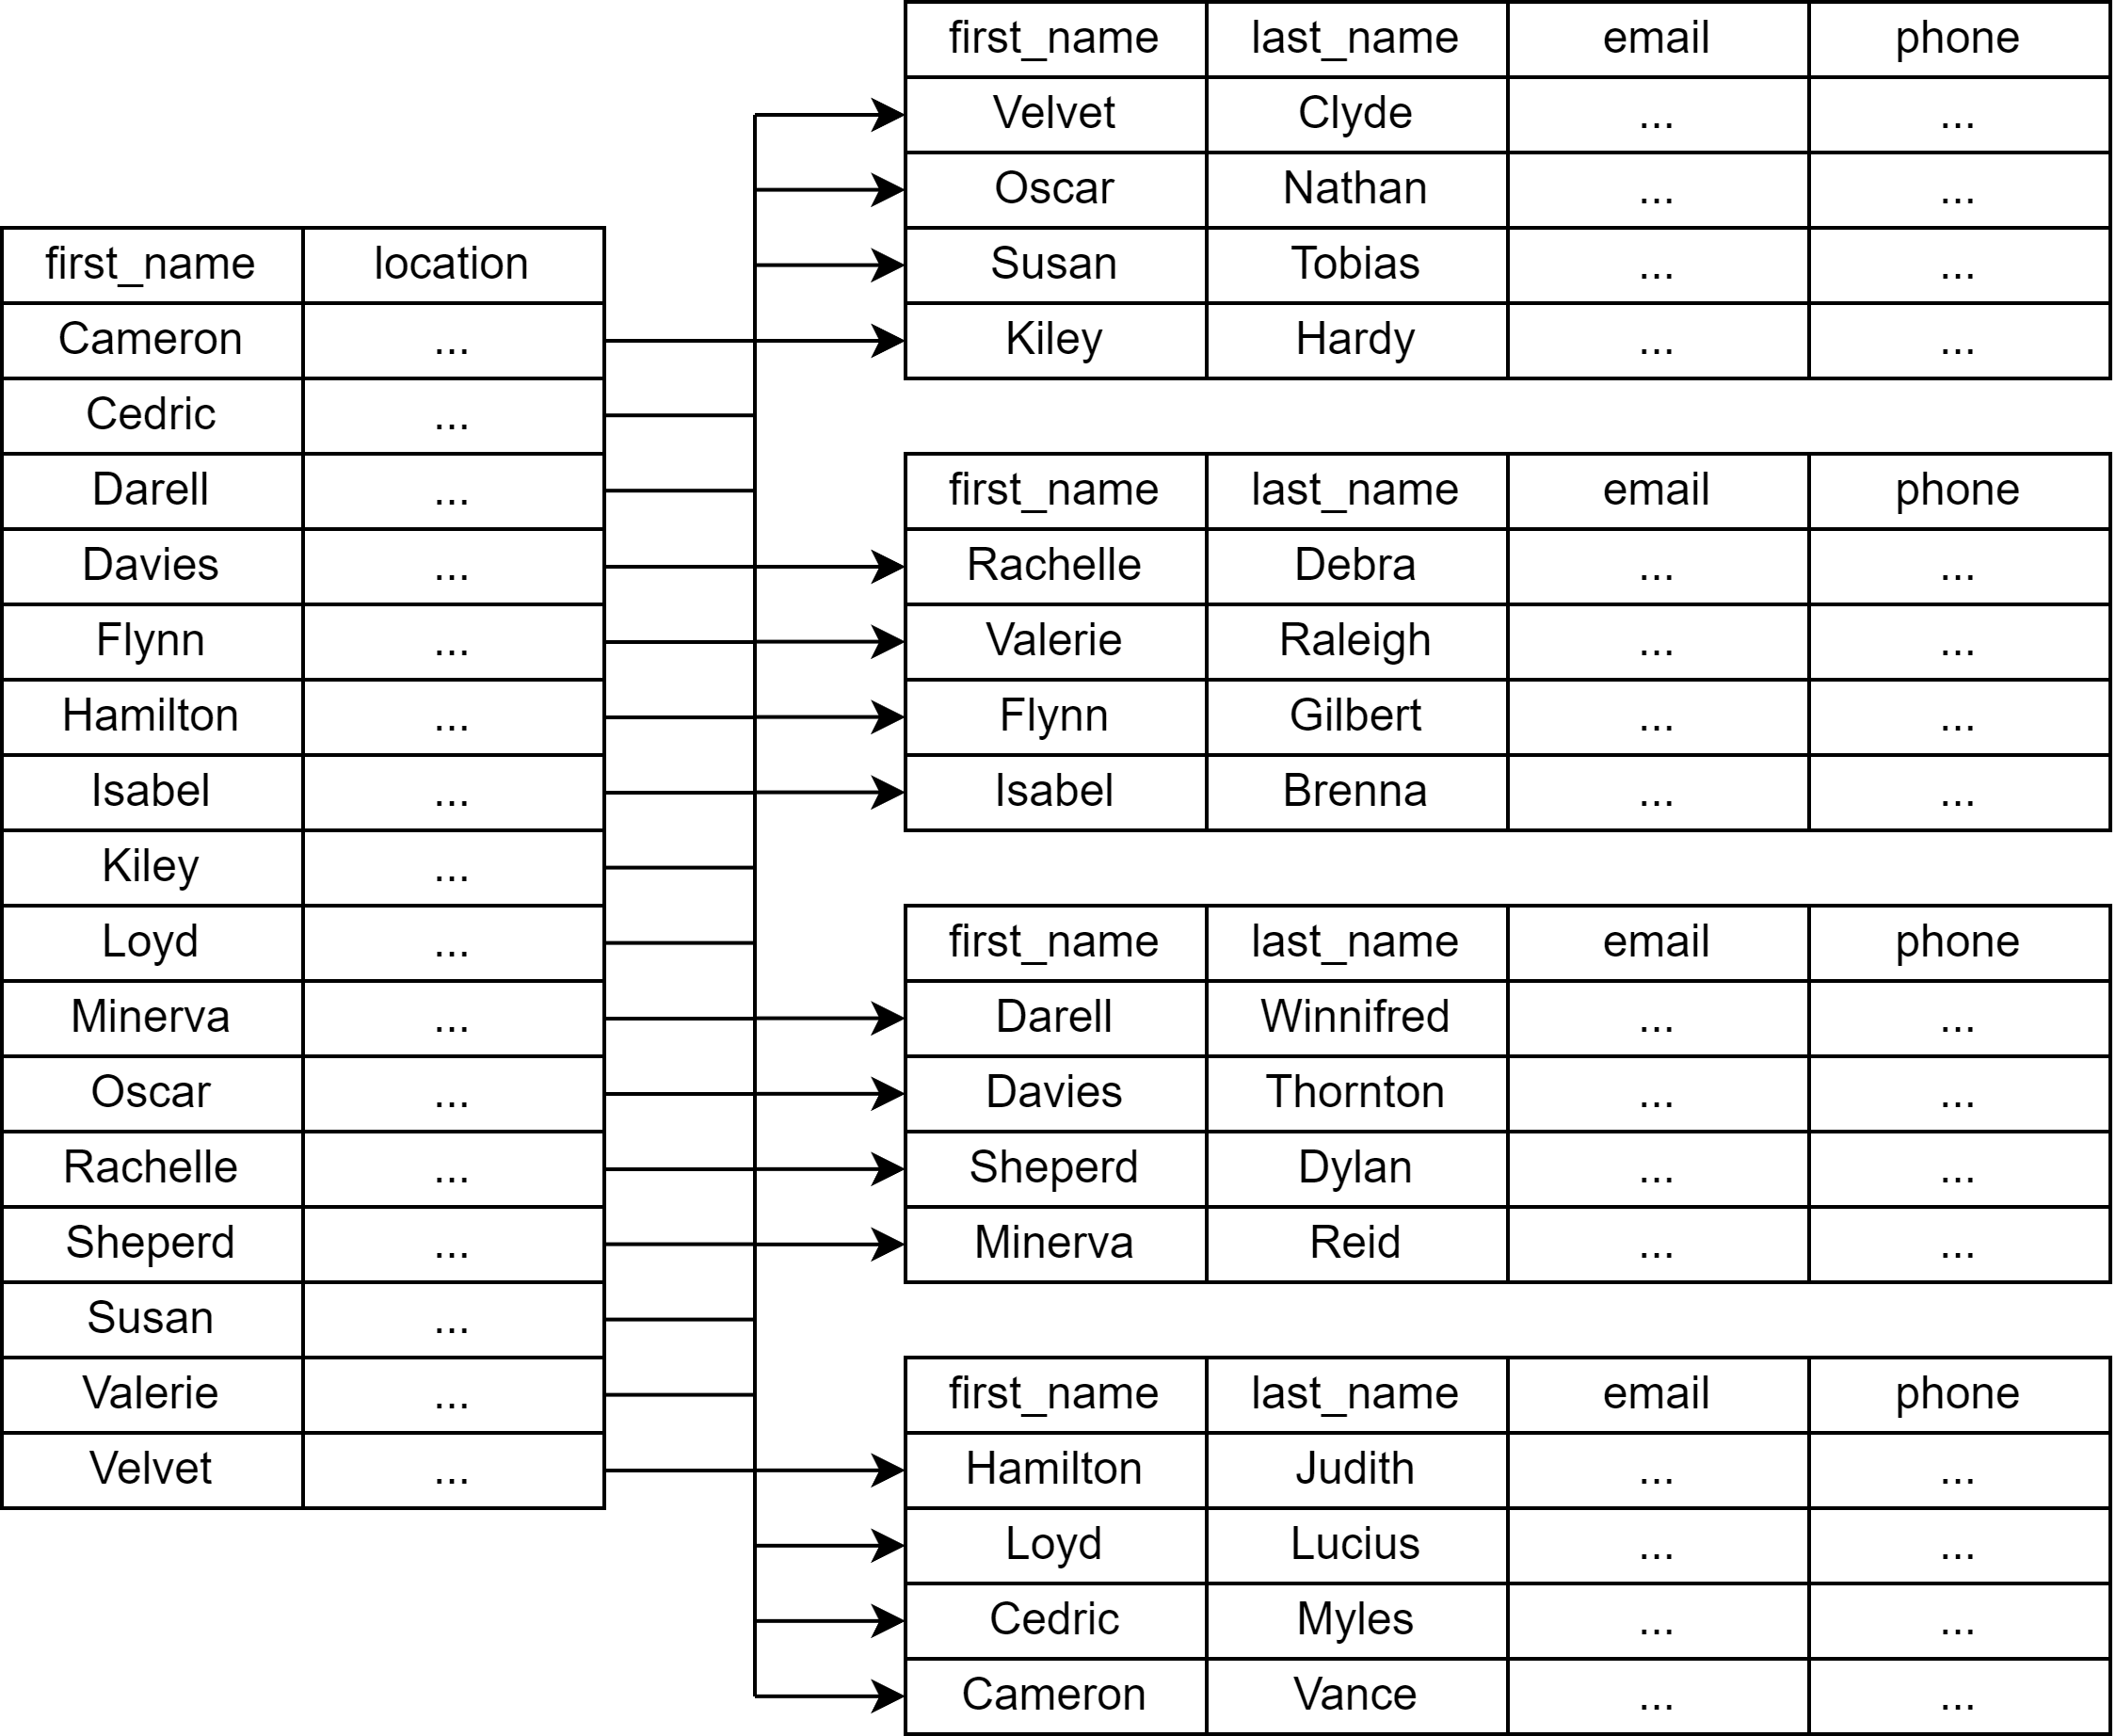
\includegraphics[width=0.5\linewidth]{images/dense.png}
    \caption{Example of dense indexing}
\end{figure} 
\begin{definition}[\textit{Sparse index}]
    An index is termed sparse when it has index entries only for some search-key values in the file (one index per block). 
\end{definition}
While this requires less space, the search process is slower as it involves scanning an entire block to find the tuple. 
Sparse indexing necessitates ordered data structures and primary indexing, providing a favorable trade-off with one index entry for each block in the file.
\begin{figure}[H]
    \centering
    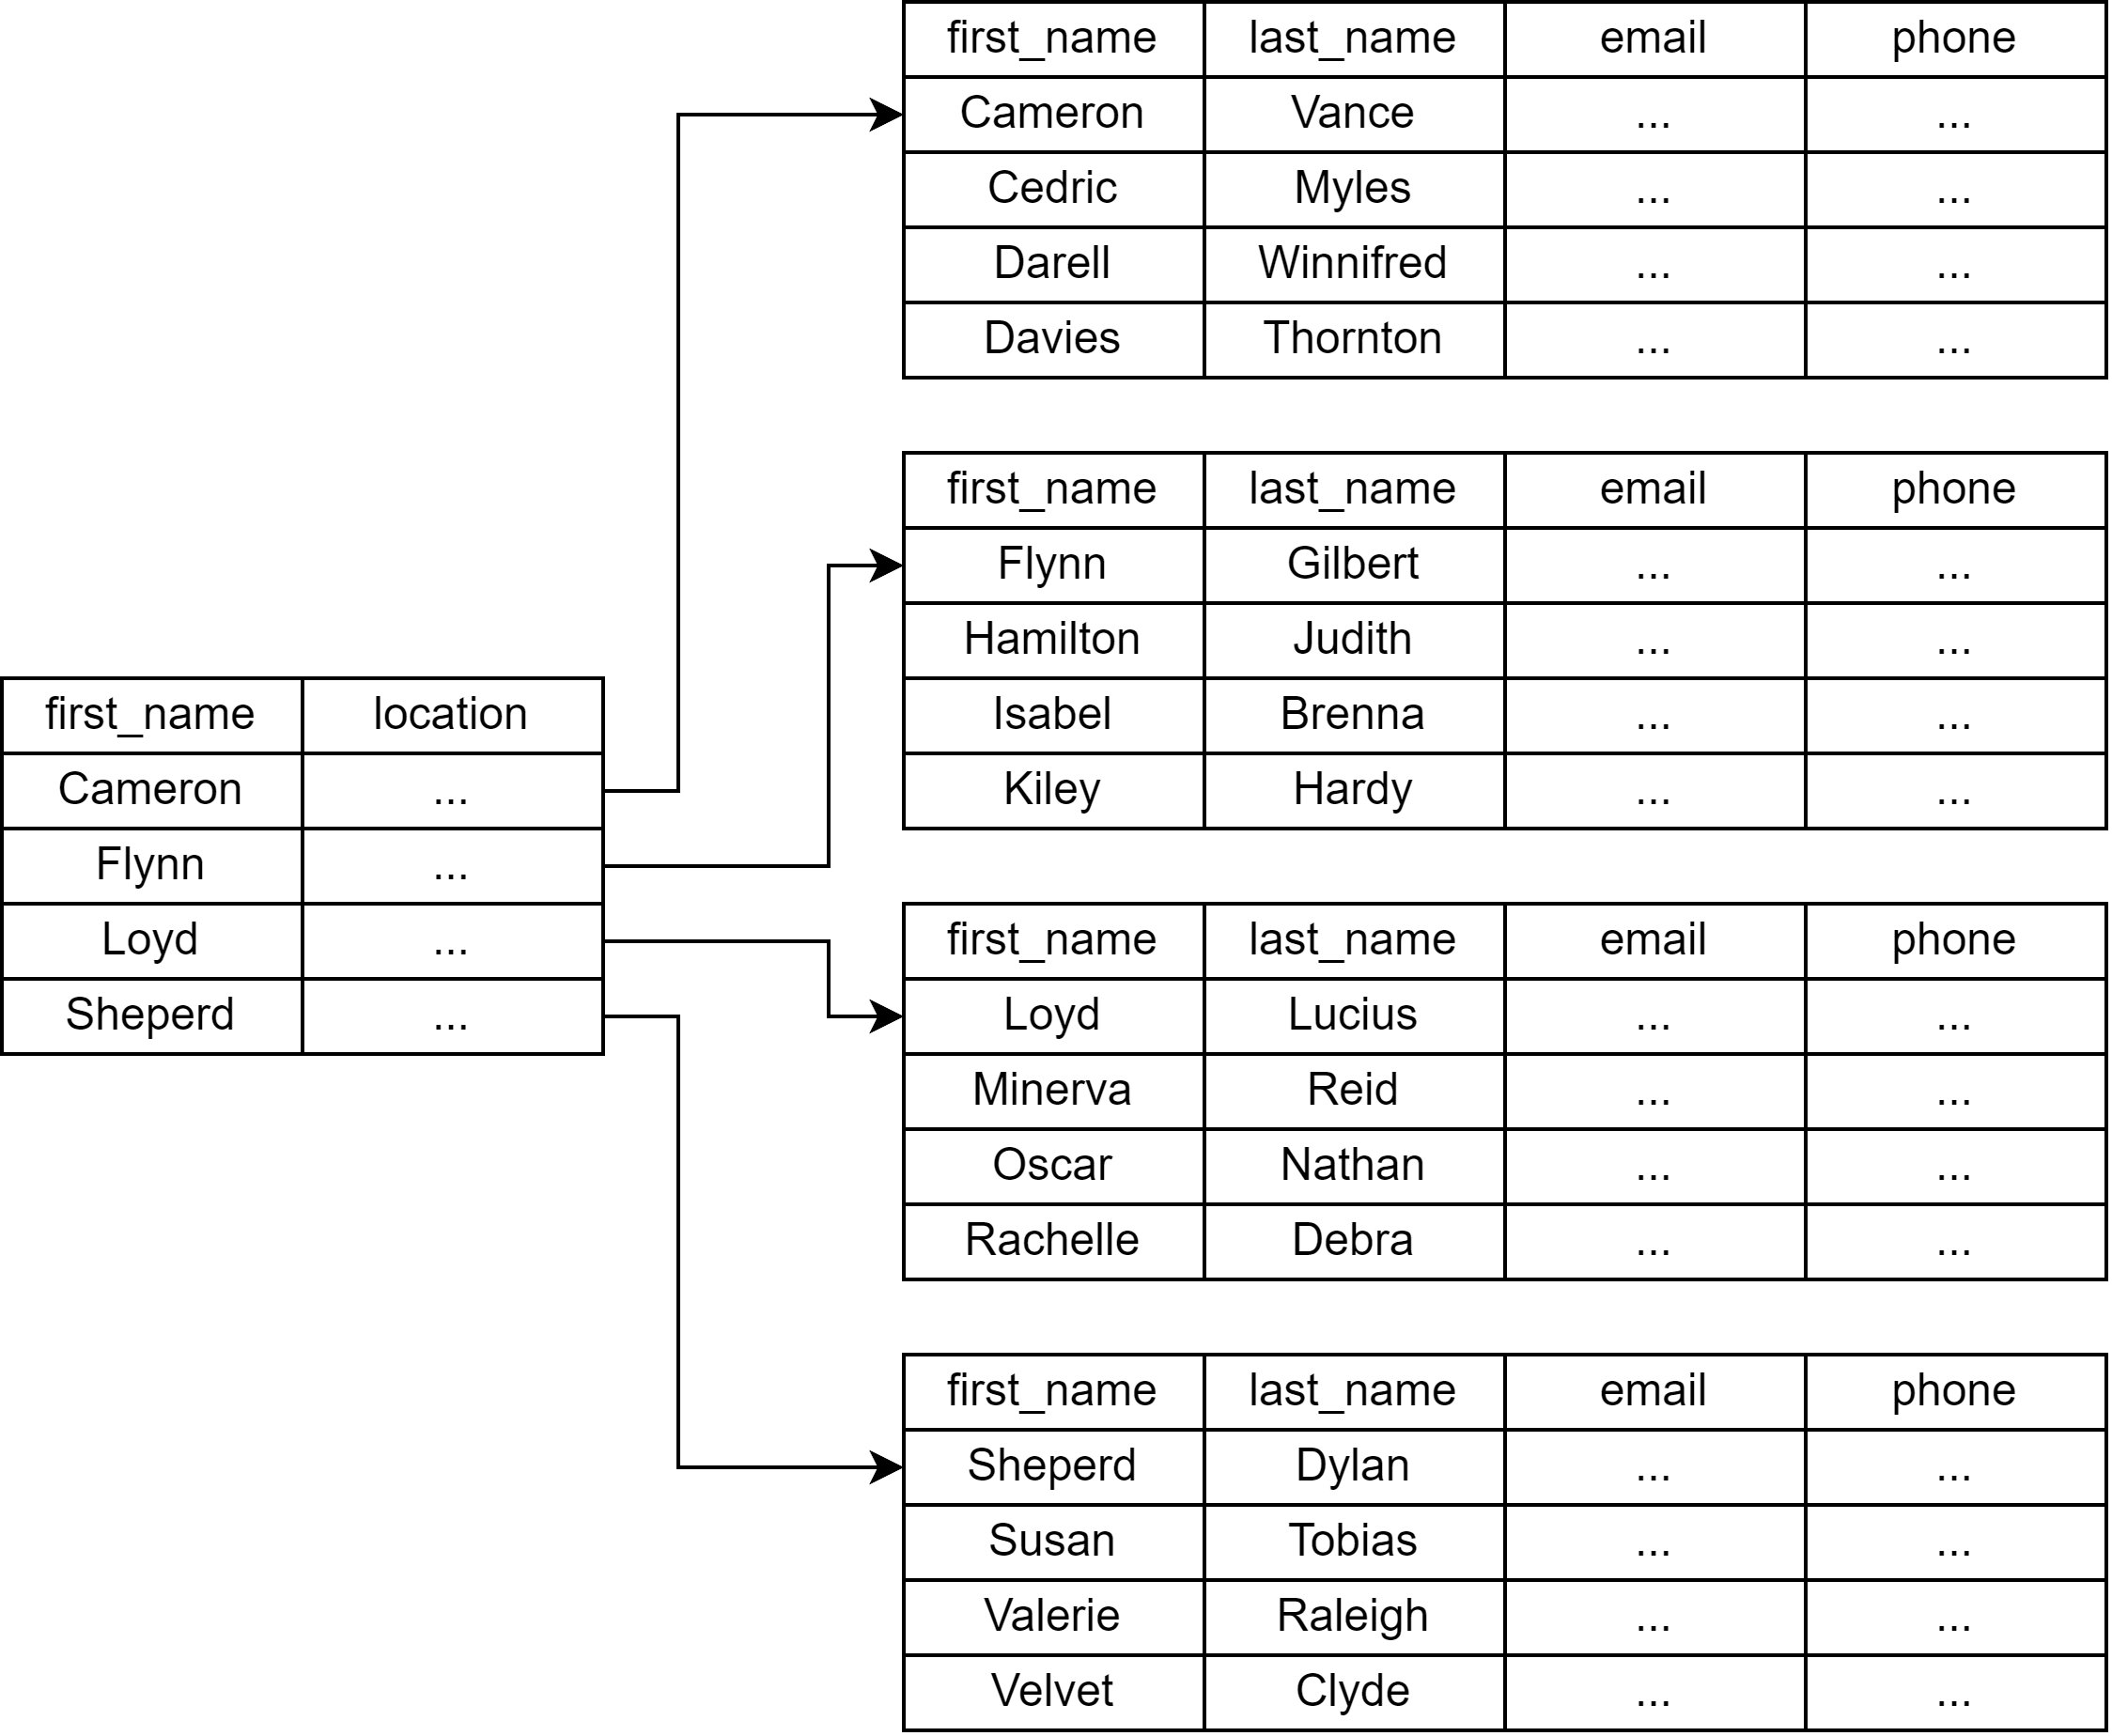
\includegraphics[width=0.5\linewidth]{images/sparse.png}
    \caption{Example of sparse indexing}
\end{figure} 

\paragraph*{Primary index}
A primary index is defined on sequentially ordered structures.
The search key (SK) is unique and coincides with the attribute according to which the structure is ordered (search key = ordering key). 
Only one primary index per table can be defined, typically on the primary key, but not necessarily. 
The primary index can be dense or sparse.

\paragraph*{Clustering index}
A clustering index is a generalization of the primary index where the ordering key may not be unique.
The pointer of key $X$ refers to the block containing the first tuple of key $X$.
It can be sparse or dense, but typically it's sparse.

\paragraph*{Secondary index}
A secondary index has a search key specifying an order different from the sequential order of the file.
Multiple secondary indexes can be defined for the same table, each on different search keys.
It is necessarily dense because tuples with contiguous values of the key can be distributed in different blocks.

\paragraph*{Summary} 
The indexes are smaller than primary data structures, so they can be loaded into primary memory. 
They efficiently support point queries, range queries, and sorted scans. 
However, they are less efficient than hash structures for point queries. 
Adding indexes to tables requires the DBMS to update each index after an insert, update, or delete operation, incurring potential costs and slowing down data-changing operations.

\paragraph*{Indexes in SQL}
To create an SQL index, every table should have:
\begin{itemize}
  \item A suitable primary storage, possibly sequentially ordered.
  \item Several secondary indexes, both unique and non-unique, on the attributes most used for selections and joins.
    Secondary structures are progressively added, checking that they are used by the system.
\end{itemize}

Guidelines for choosing indexes:
\begin{enumerate}
  \item Do not index small tables. 
  \item Index the primary key of a table only if it is not a key of the primary file organization.
  \item Add a secondary index to any column heavily used as a secondary key.
  \item Add secondary index structures on columns involved in \texttt{SELECT} or \texttt{JOIN} criteria, \texttt{ORDER BY}, \texttt{GROUP BY}, and other operations involving sorting.
  \item Avoid indexing a column or table that is frequently updated.
  \item Avoid indexing a column if the query will retrieve a significant number of rows.
  \item Avoid indexing columns that consists of long strings.
\end{enumerate}

The SQL commands used to create and remove the indexes are as follows: 
\begin{lstlisting}[style=SQL]
CREATE [UNIQUE] INDEX <index_name> ON <table_name>[(<column_name>, ...)]
DROP INDEX <index_name>
\end{lstlisting}

\subsection{Tree-based structures}
Frequently used in relational DBMSs (DBMS) for secondary index structures, balanced trees support associative access based on the value of a key search field.
These trees are specifically balanced in that the lengths of the paths from the root node to the leaf nodes are all equal, contributing to enhanced performance. 
There are two main types of balanced trees used in this context:
\begin{itemize}
    \item \textit{B trees}: key values are stored in both internal and leaf nodes.
    \item \textit{B+ trees}: all key values are stored only in leaf nodes.
\end{itemize}

\paragraph*{B+ trees}
The B+ tree is an evolution from the B-tree, with each node stored in a block. 
Key values are exclusively stored in the leaf nodes, making B+ trees more efficient than B-trees, especially when a majority of the nodes are leaves. 
The fan-out of B+ trees depends on the size of the block, the key, and the pointer.

\paragraph*{Internal node's structure}
Each node contains $F$ keys, sorted lexicographically, and $F+1$ pointers to child nodes.
Each key $K_j, \: 1 \leq j \leq F$ is followed by a pointer $P_j$, with  $K_1$ preceded by a pointer $P_0$.
Each pointer addresses a subtree, with $P_0$ pointing to the subtree containing keys less than $K_1$, $P_F$ pointing to the subtree containing keys greater or equal to $K_F$, and intermediate pointers addressing subtrees containing keys $K$ within the interval $K_j \leq K < K_{j + 1}$.
The value of $F$ depends on the size of the page and the amount of space occupied by the key values and the pointers.
\begin{figure}[H]
    \centering
    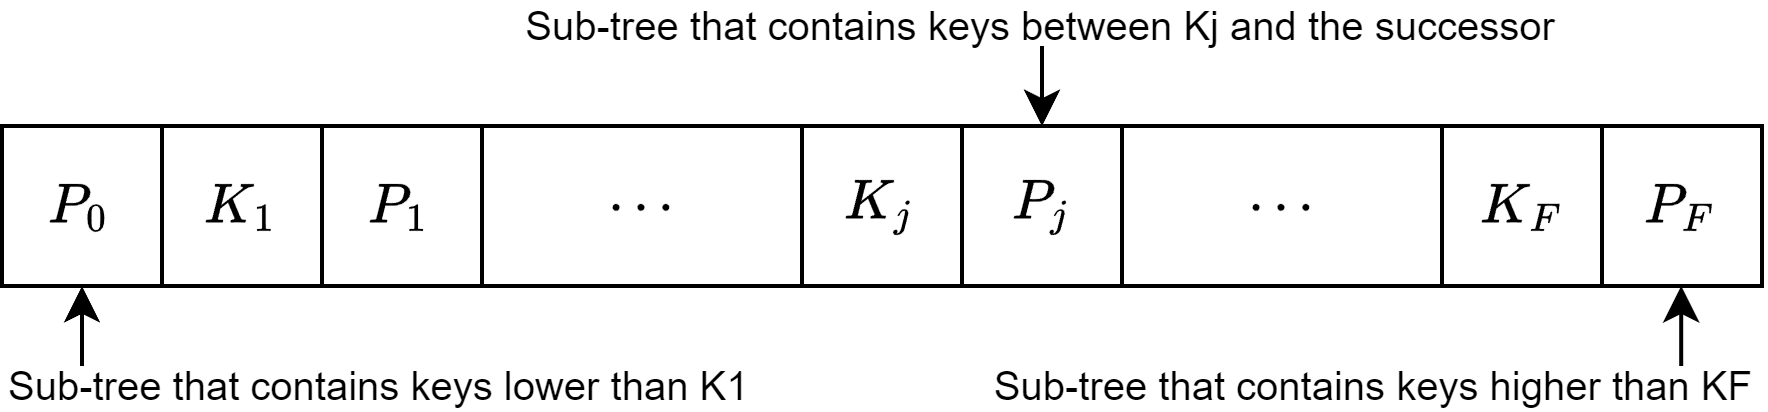
\includegraphics[width=0.75\linewidth]{images/int.png}
    \caption{Structure of an internal node}
\end{figure} 

\paragraph*{Leaf node's structure}
The leaf node's structure resembles that of an internal node but contains only pointers to data tuples or the data tuples themselves. 
Leaf nodes can be structured in two ways:
\begin{enumerate}
  \item The leaf node contains the entire tuple, making it key-sequenced.
  \item The leaf node contains pointers to blocks of the database that contain tuples with the same key value, making it indirect.
\end{enumerate}
\begin{figure}[H]
    \centering
    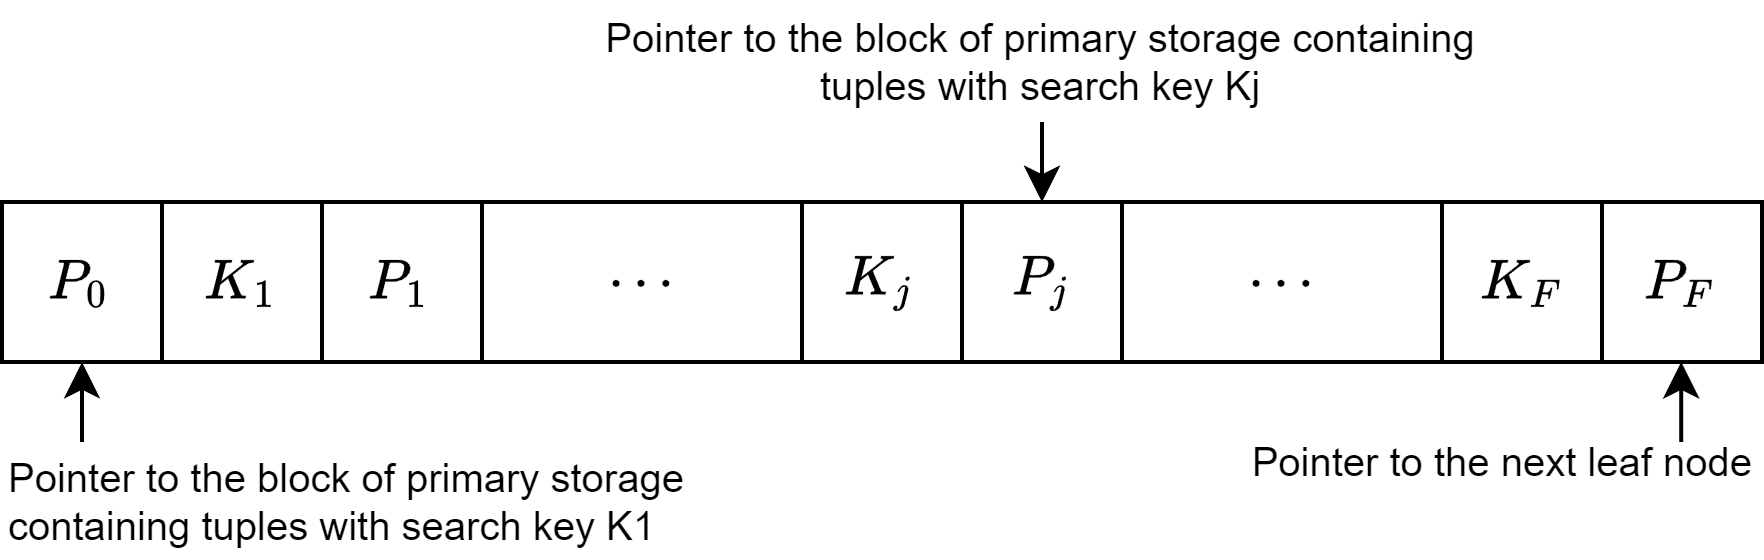
\includegraphics[width=0.75\linewidth]{images/ext.png}
    \caption{Structure of a leaf node}
\end{figure} 

\paragraph*{Search Mechanism}
The search mechanism involves following pointers starting from the root. 
At each intermediate node:
\begin{itemize}
  \item If $V < K_1$, follow the pointer $P_0$.
  \item If $V \geq K_F$, follow the pointer $P_F$.
  \item Otherwise, follow the pointer $P_j$ such that $K_j \leq V < K_{j + 1}$. 
\end{itemize}
The search continues until a leaf node is found. 
In a key-sequenced leaf node, the search is complete as the tuple is found. 
In an indirect leaf node, it's necessary to access the memory block pointed to by the pointer $P_j, \: 0 \leq j \leq F$.


\paragraph*{Differences}
B+ trees have linked leaf nodes through a chain of pointers, ordered by key values. 
This chain enables efficient execution of range queries, allowing sequential scanning of leaves for values within a given range. 
This ordered scan is not possible in B trees, where accessing tuples in a specific range requires a search for each tuple. 
B trees use two pointers for each value  $k_i$ in intermediate nodes, saving space in the index pages and terminating the search when a key value is found without continuing the search in subtrees.